\documentclass[12pt,a4paper]{article}

% Packages
\usepackage[utf8]{inputenc}
\usepackage{amsmath,amssymb}
\usepackage{graphicx}
\usepackage{geometry}
\usepackage{listings}
\usepackage{hyperref}

% Page Layout
\geometry{margin=1in}
\setlength{\parindent}{1cm}

% Code Listing Style
\lstset{basicstyle=\ttfamily, frame=single, breaklines=true, captionpos=b}

% Title Page Info
\title{Real Time Signal Processing for Proximity Sensor Data}
\author{Group 04: Uğur ÖZKAN(21050161003), Eren YILMAZ(22050151024), Semih MERT (22050171003), Name4, Name5}
\date{\today}

\begin{document}

\maketitle
\section{Abstract}

The increasing capabilities of autonomous UAVs have led to remarkable feats such as drone racing and aerial acrobatics. However, fundamental tasks like obstacle detection and avoidance remain challenging, especially in scenarios involving the focus of expansion where optic flow is minimal. This difficulty is exacerbated in real-world environments with dynamic lighting conditions, creating a need for robust datasets to benchmark and develop solutions. This paper introduces the Obstacle Avoidance Dataset for Drones, which provides real indoor environment data collected with aerial robotics sensors. The dataset focuses on detecting obstacles around the focus of expansion and includes over 1300 samples under varied conditions of lighting and obstacle placement. Equipped with sensors like an event-based camera, an RGB camera, a 24-GHz radar, and a 6-axes IMU, the dataset also incorporates ground truth position and attitude data from the OptiTrack motion capture system. Data is available in multiple formats, enabling benchmarking of algorithms for obstacle detection, avoidance, and autonomous navigation.

\section{Introduction}

Unmanned Aerial Vehicles (UAVs) have advanced significantly, performing tasks ranging from autonomous drone racing—as seen in challenges like AlphaPilot 2019—to intricate maneuvers such as crossing windows or executing aerial acrobatics. Despite these achievements, one of the most essential tasks for drones, obstacle detection and avoidance, remains notably difficult to accomplish autonomously. This challenge is rooted in the complexity of detecting obstacles in the focus of expansion, where the optic flow approaches zero. The problem becomes even more pronounced in real-world scenarios with abrupt changes in light intensity, further hindering the robustness of autonomous systems.

Obstacle detection and avoidance is critical for UAVs in various real-life applications, including search and rescue missions, package delivery, and autonomous surveillance. The lack of robustness in this area poses risks to both UAVs and their surroundings. Addressing these challenges requires datasets that simulate real-world conditions and provide high-fidelity data for testing algorithms.

To bridge this gap, the Obstacle Avoidance Dataset for Drones was developed. This dataset focuses on obstacle detection near the focus of expansion and offers data collected in an indoor flying arena under controlled conditions. The setup features a Micro Aerial Vehicle (MAV) equipped with advanced sensors such as an event-based camera, a 6-axes IMU, a 24-GHz radar, and a full HD RGB camera. The dataset includes ground truth data provided by the OptiTrack motion capture system, ensuring accurate benchmarking. With 1369 trials recorded under different lighting and obstacle conditions, this dataset serves as a valuable resource for researchers and developers aiming to improve UAV navigation and obstacle avoidance capabilities.

The MAV operates within the Cyber Zoo at TU Delft, a specialized flying arena, and data collection is managed via a ROS environment running on an onboard Odroid XU4 system. Trials involve navigating through one or two obstacles under full light (100 Lux) or dim light (1-3 Lux) conditions. The dataset, provided in both ROS bag and CSV formats, includes raw sensor data and ground truth, alongside RGB camera footage. This comprehensive collection supports the development of robust, multi-sensory solutions for autonomous navigation and obstacle avoidance, offering a foundation for future innovations in aerial robotics.


\section{Methodology}

This section describes the approaches and techniques used for processing and visualizing multi-sensor data from various sensing modalities.

\subsection{Data Collection and Processing}

The analysis pipeline processes data from five different sensor types:

\begin{itemize}
    \item RGB Camera Data: Video frames are sampled at intervals of 30 frames to obtain key visual information, with a maximum of 5 frames collected for visualization purposes.
    
    \item Dynamic Vision Sensor (DVS): Event-based vision data is processed with parameters DIMX = 240 and DIMY = 180 at 24 FPS. Events are accumulated into frames with polarity-based color coding (red for negative events, blue for positive events).
    
    \item OptiTrack Motion Capture: Position data (x, y, z) and orientation quaternions (a, b, c, d) are collected and time-synchronized with other sensor streams. The data provides ground truth trajectory information.
    
    \item Inertial Measurement Unit (IMU): Linear accelerations and angular velocities are processed in three axes. A moving average filter with window size W = 15 is applied to reduce noise:
    
    \begin{equation}
        x_{filtered}[n] = \frac{1}{W}\sum_{i=0}^{W-1} x[n+i]
    \end{equation}
    
    \item Radar: Two-antenna radar data is processed using Fast Fourier Transform (FFT) analysis. The processing includes:
    \begin{enumerate}
        \item Zero-padding the chirp signals for improved FFT performance
        \item Computing complex FFT for both receive channels
        \item Extracting magnitude and phase information
    \end{enumerate}
\end{itemize}

\subsection{Data Synchronization and Visualization}

All sensor streams are temporally aligned using timestamps normalized to seconds. The visualization pipeline includes:

\begin{enumerate}
    \item Time-series plots for OptiTrack position and orientation data
    \item Filtered and unfiltered IMU measurements visualization
    \item 2D trajectory plot with obstacle locations marked as circles
    \item 3D trajectory visualization with cylindrical obstacles
    \item Radar FFT analysis showing magnitude and phase information
\end{enumerate}

\subsection{Signal Processing Techniques}

Several signal processing methods are employed:

\begin{equation}
    FFT_{radar}(re, im) = \{\mathcal{F}(re + j\cdot im)\}
\end{equation}

The magnitude and phase are computed as:

\begin{equation}
    magnitude = \sqrt{real^2 + imag^2}
\end{equation}

\begin{equation}
    phase = \arctan2(real, imag)
\end{equation}

For the radar processing, we implement:
\begin{itemize}
    \item Zero-padding to improve frequency resolution
    \item FFT shift for centered frequency representation
    \item Complex signal processing for both radar channels
\end{itemize}

\subsection{Coordinate Systems and Transformations}

The system uses multiple coordinate frames:
\begin{itemize}
    \item OptiTrack world coordinate system for absolute positioning
    \item IMU body-fixed coordinate frame for acceleration and angular velocity
    \item Image coordinates for DVS (240×180 pixels) and RGB camera data
\end{itemize}

\subsection{Implementation Details}

The implementation utilizes several Python libraries:
\begin{itemize}
    \item NumPy for numerical computations and array operations
    \item Matplotlib for visualization and plotting
    \item OpenCV (cv2) for RGB video processing
    \item PIL for image processing
    \item SciPy for FFT computations and signal processing
\end{itemize}

The visualization framework is designed to provide comprehensive insight into the sensor fusion dataset, enabling analysis of both spatial and temporal relationships between different sensor modalities.
\section{Data and Implementation}
\textbf{Briefly describe the dataset, preprocessing steps, and Python implementation. Include a code snippet if relevant:}

The dataset contains data from various sensors stored in CSV format. Preprocessing includes filtering noise and normalizing time series. For example, radar data undergoes FFT for frequency domain analysis, while IMU data uses sliding window filters for smoothing.

\begin{lstlisting}[language=Python, caption=Radar Data undergoes FFT]
import numpy as np
from scipy.fft import fft, fftshift

def fft_radar(re, im):
    s1 = fftshift(fft(re))
    s2 = fftshift(fft(im))
    magnitude = np.sqrt(s1.real**2 + s2.imag**2)
    return magnitude

# Load radar sample
radar_data = np.loadtxt('sample_radar.csv', delimiter=',')
real_part = radar_data[:, 1]
imag_part = radar_data[:, 2]
magnitude = fft_radar(real_part, imag_part)

\end{lstlisting}
\section{Results and Discussion}
\textbf{Present findings with graphs or screenshots:}

Using the provided scripts, radar data visualization showcases signal magnitude and phase for obstacle detection. IMU data plots reveal smoothed accelerations and angular velocities, supporting movement dynamics analysis. Below is an example visualization of FFT magnitude for radar data and smoothed IMU signals:

Graphs:

Radar FFT magnitude plot: Peaks indicate obstacle presence at specific distances.
IMU filtered accelerations: Smooth curves represent stability and noise reduction.
\begin{figure}[h!]
    \centering
    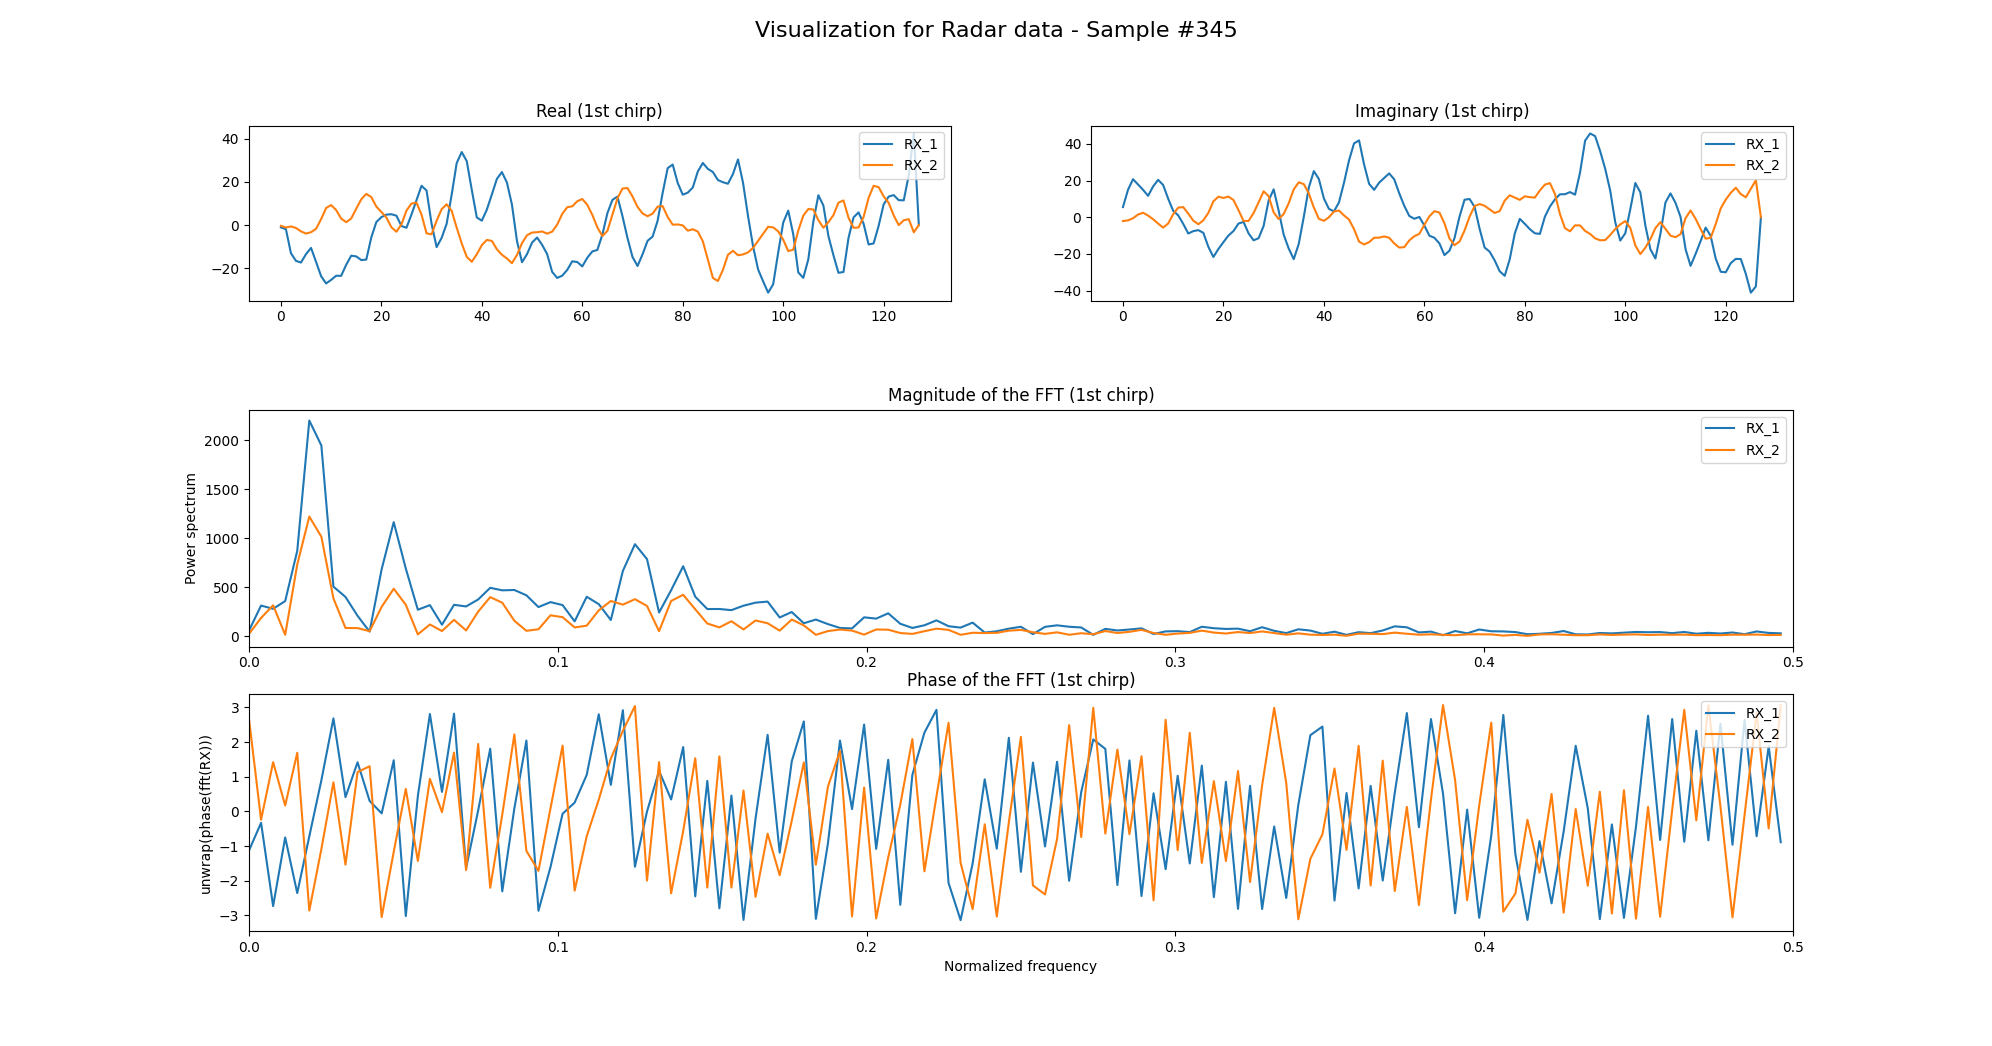
\includegraphics[width=0.8\textwidth]{radar_sample_345.png} 
    \caption{This is the graph of radar sample 345.}
    \label{fig:Radar_sample_345}
\end{figure}

\section{Conclusion}
\textbf{Summarize key outcomes and suggest future improvements.}

\section*{References}
\begin{itemize}
    \item \url{https://github.com/bilgivecesaret/Real-Time-Signal-Processing-for-Proximity-Sensor-Data}
    \item \url{https://github.com/JuSquare/ODA_Dataset/tree/master}
    \item \url{https://www.lockheedmartin.com/en-us/news/events/ai-innovation-challenge.html}
    \item \url{https://data.4tu.nl/articles/dataset/The_Obstacle_Detection_and_Avoidance_Dataset_for_Drones/14214236/1}
    \item  \url{https://www.roboticsproceedings.org/rss16/p040.pdf}
    \item \url{https://www.liebertpub.com/doi/full/10.1089/soro.2017.0120}   
\end{itemize}

\end{document}

